\documentclass[tikz,border=10pt]{standalone}
\usepackage{tikz}
\usetikzlibrary{shapes,arrows,positioning,fit,shadows}

\begin{document}
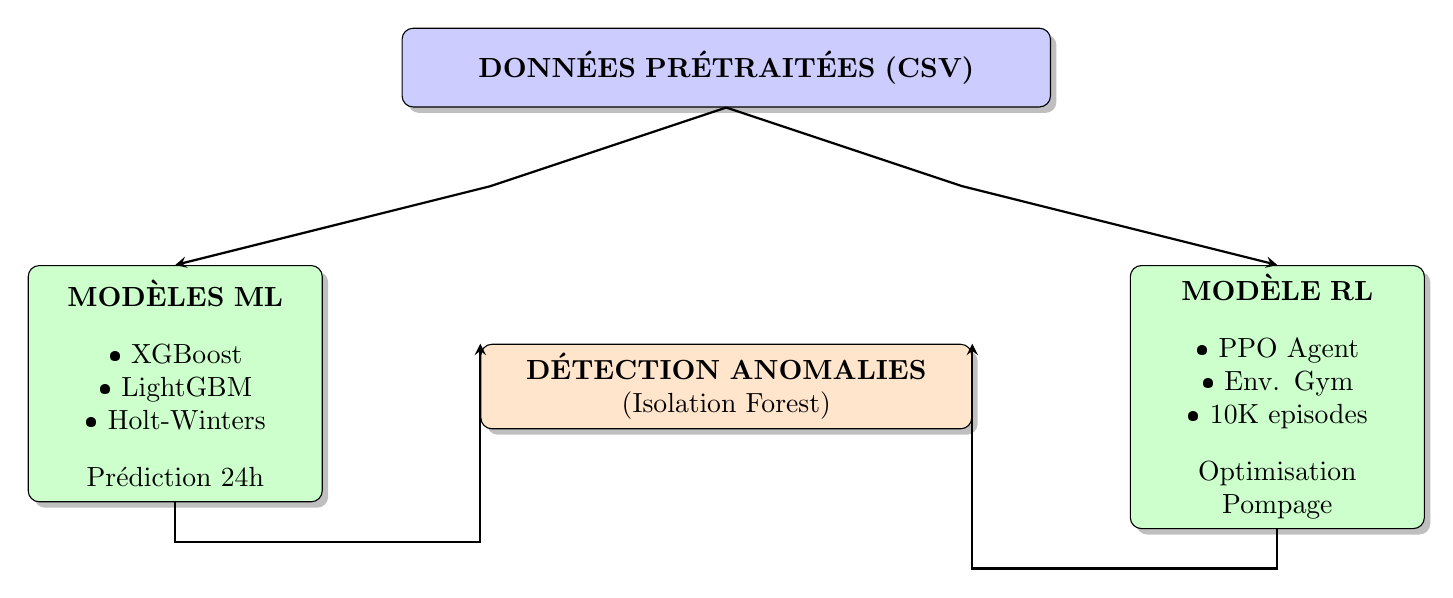
\begin{tikzpicture}[
    node distance=1.5cm,
    box/.style={rectangle, draw, fill=blue!20, text width=8cm, text centered, rounded corners, minimum height=1cm, drop shadow},
    mlbox/.style={rectangle, draw, fill=green!20, text width=3.5cm, text centered, rounded corners, minimum height=3cm, drop shadow},
    detbox/.style={rectangle, draw, fill=orange!20, text width=6cm, text centered, rounded corners, minimum height=1cm, drop shadow},
    arrow/.style={->, >=stealth, thick}
]

% Top box - Data
\node[box] (data) at (0,0) {
    \textbf{DONNÉES PRÉTRAITÉES (CSV)}
};

% ML Models - Left
\node[mlbox, below left=2cm and 1cm of data] (ml) {
    \textbf{MODÈLES ML}\\[0.3cm]
    • XGBoost\\
    • LightGBM\\
    • Holt-Winters\\[0.3cm]
    Prédiction 24h
};

% RL Model - Right
\node[mlbox, below right=2cm and 1cm of data] (rl) {
    \textbf{MODÈLE RL}\\[0.3cm]
    • PPO Agent\\
    • Env. Gym\\
    • 10K episodes\\[0.3cm]
    Optimisation\\
    Pompage
};

% Anomaly Detection - Bottom
\node[detbox, below=3cm of data] (anom) {
    \textbf{DÉTECTION ANOMALIES}\\
    (Isolation Forest)
};

% Arrows
\draw[arrow] (data.south) -- ++(-3,-1) -- (ml.north);
\draw[arrow] (data.south) -- ++(3,-1) -- (rl.north);
\draw[arrow] (ml.south) -- ++(0,-0.5) -| (anom.north west);
\draw[arrow] (rl.south) -- ++(0,-0.5) -| (anom.north east);

\end{tikzpicture}
\end{document}
